\begin{enumerate}[label=\thesection.\arabic*.,ref=\thesection.\theenumi]
\numberwithin{equation}{enumi}

\item For a Transfer function G\brak{s} in unity negative feedback ,whose error  $K_v$ = 2. Determine K 
\begin{align}
G\brak{s} &= \frac{K}{s\brak{s+2}\brak{s+4}\brak{s+6}}
\label{eq:ee18btech11049_system}
\end{align}




\solution For unity feedback we have Velocity error constant $\brak{K_v}$

\begin{align}
K_v &= \lim_{s \to 0} s G\brak{s} 
\end{align}
\begin{align}
\lim_{s \to 0} \brak{\frac{K}{\brak{s+2}\brak{s+4}\brak{s+6}} }& = 2 \\
\implies K = 96
\end{align}
It's Phase Margin  = 19\degree\\
and Gain Crossover Frequency = 1.49 rad/s

\item Design a lead Compensator to yield a Phase margin of 30\degree \\
\solution So ,we need a phase lead of 11 at the gain crossover frequency, Using a lead Compensator C\brak{s}.
\begin{align}
    C\brak{s} &= \frac{\brak{s+a_1}}{\brak{s+a_2}}
\end{align}{}
Now choose $a_1$ and $a_2$ \brak{a_1 < a_2} such that, phase lead of Compensator is 11, and has negligible gain.
\begin{align}
    a_1 = 1.28\\
    a_2 = 1.6
\end{align}


Refer Fig\ref{fig:total} for plot C\brak{s}.
\begin{lstlisting}
codes/ee18btech11049/lead.py
\end{lstlisting}

\begin{figure}[!h]
\centering
  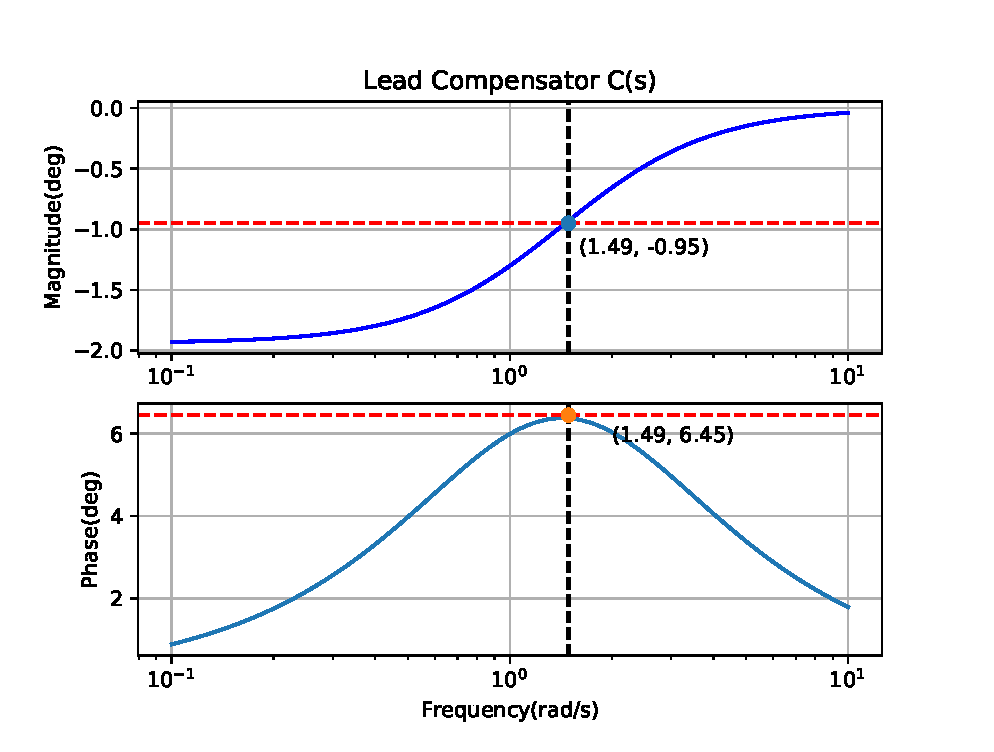
\includegraphics[width=\columnwidth]{./figs/ee18btech11049/lead.eps}
  \caption{}
  \label{fig:lead}
\end{figure}
\item Plot overall graph after adding lead compensator.
Refer Fig\ref{fig:lead} for plot C\brak{s}G\brak{s}.
\begin{lstlisting}
codes/ee18btech11049/full.py
\end{lstlisting}
\begin{figure}[!h]
\centering
  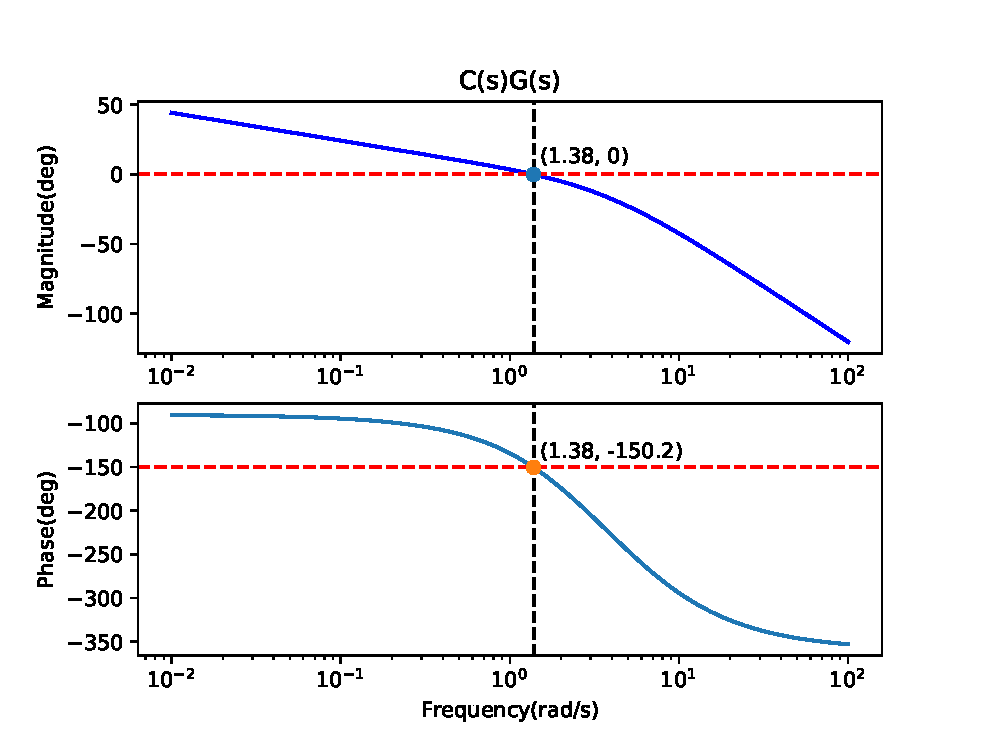
\includegraphics[width=\columnwidth]{./figs/ee18btech11049/full.eps}
  \caption{}
  \label{fig:total}
\end{figure}



\textbf{NOTE :} Overall Gain is definitely changed by Lead compensator, which increases gain crossover frequency. This points should be noted while designing a controller, and parameters to be changed accordingly to get exact results.











\end{enumerate}     
